\documentclass[10pt, a4paper]{beamer}
%\documentclass{article}

%Metadaten
\title{Machine Vision with Arduino Portenta H7}

\subtitle{Face recognition using Edge Impulse and Arduino PortentaH7 connected to Vision Shield.}
%\institution{University of Applied Science Hochschule Emden/Leer}
\author{Vatsal Mahajan, Manoj Selvaraju, Vijay Singh}

%\date{\today}
\date{\today}

% siehe hesader.tex Zeile 10-16 zum Aktivieren der Notes
% Kommentare stehen in \notes{} und können im 2-screen-mode genutzt werden
%%%%%%
%
% $Autor: Wings $
% $Datum: 2020-01-18 11:15:45Z $
% $Pfad: githubtemplate/Template/Presentations/Template/slides/header.tex $
% $Version: 4620 $
%
%
% !TeX encoding = utf8
% !TeX root = Rename
%
%%%%%%


%Packages
\usepackage[utf8]{inputenc} %Für Umlaute, da BibLaTeX
\usepackage[german]{babel}
\usepackage{amsmath}
\usepackage{amsfonts}
\usepackage{amssymb}
\usepackage{colortbl}
\usepackage{cancel} %'\cancel{}', '\bcancel{}' und '\xcancel{}'

%%%%%%%%%2-Screen%%%%%%%%%%%%%%%%%%%%%%%%%%%%%%%%%%%%%%%%%%%%
\usepackage{pgfpages} 
%%%%Kommentiert für Beamer
%%%%Aktiv für Notes
%\setbeameroption{show notes on second screen=bottom}
%\setbeameroption{second mode text on second screen=bottom}
%%%%%%%%%%%%%%%%%%%%%%%%%%%%%%%%%%%%%%%%%%%%%%%%%%%%%%%%%%%%%

%Für Grafiken
\usepackage{tikz}
\usetikzlibrary{mindmap}
\usepackage{gnuplottex}
\usepackage{pgf}
\usepackage{colortbl} 
\usetikzlibrary{calc}
\usetikzlibrary{shapes,arrows} %Für Flowchart
\usetikzlibrary{shapes.geometric} %Für Flowchart
\usepackage{scalefnt}
\usetikzlibrary{decorations.markings} %Für => pfeile
\usetikzlibrary{calc,patterns,decorations.pathmorphing,decorations.markings}
%Für urls in Quellen
\usepackage{url}
%Für Diagramme (autotools)
%\usepackage{graphicx}
%\usepackage{graphviz}

%\usepackage[
%  backend=biber,
%  style=alphabetic,
%  sorting=ynt
%]{biblatex}

\usepackage[natbib=true,style=alphabetic,backend=bibtex,useprefix=true]{biblatex}

%Formatierungen
\mode<presentation>
\setbeamertemplate{headline} 
{%
\begin{beamercolorbox}[rounded=true, center]{bgcolor}
\begin{columns}[T]
\begin{column}{9cm}
{\color{gray}\begin{tiny}Hochschule Emden/Leer\end{tiny}} \\ 
{\color{gray}\begin{tiny}Department of Electrical and Computer Engineering\end{tiny}} \\ 
{\color{gray}\begin{tiny}Industrial Informatics\end{tiny}} \\
%{\color{gray}\begin{tiny}Innovationsforum MSR\end{tiny}}
\end{column}
\begin{column}{2cm}

\includegraphics[scale=0.25]{img/technik.jpg}
\end{column}
\end{columns}
\end{beamercolorbox}
 }
\insertsectionhead
\insertsubsectionhead
\usetheme{default}
\useinnertheme[shadow=true]{rounded}
\usebackgroundtemplate
{%
      \rule{0pt}{\paperheight}%
      \hspace*{\paperwidth}%
      \makebox[0pt][r]{
\includegraphics[width=\paperwidth]{img/hintergrund2.png}}
 }

\definecolor{HSELhellblau}{RGB}{138,198,203}
\definecolor{HSELblau}{RGB}{0,59,95}
\usecolortheme[named=HSELblau]{structure}
 \newcommand{\topline}{%
  \tikz[remember picture,overlay] {%
    \draw[HSELhellblau] ([yshift=-0.9cm]current page.north west)
             -- ([yshift=-0.9cm,xshift=\paperwidth]current page.north west);}}
\setbeamertemplate{section}[numbered]


\newcommand{\STANDARD}[2]
{
  \mode<presentation>%
  {%
     \begin{frame}[allowframebreaks]{#1} #2 \end{frame}
  }%
  \mode<article>
  {
    \fcolorbox{AliceBlue}%{Bisque} %{BlanchedAlmond}
    {LightGrey} %{Beige}   %{AliceBlue}
    {
      \begin{minipage}{\textwidth}{\bf #1} #2  \end{minipage}
      
      
    }%
    
    \medskip
    \hrulefill
  }
}

\newcommand{\MYNOTE}[1]
{
  \mode<presentation>%
  {%
     %\note{#1}
     \only<article>{#1}
  }%
  \mode<article>
  {
    #1
  }
}

% ------------
% sectionframe
% ------------
%
% #1  Der Name der section.
%
\newcommand{\sectionframe}[1]%
{%
	\begin{frame}
		\Huge
		\begin{center}
			#1 
		\end{center}
	\end{frame}%
}

\newcommand{\Mysection}[1]%
{%
  \section{#1}%
  
  \sectionframe{#1}%
}

\usepackage{listings}

% Farben für Syntax-Highlighting
\definecolor{dkgreen}{rgb}{0,.6,0}
\definecolor{dkblue}{rgb}{0.655,0.113,.364}
\definecolor{dkyellow}{cmyk}{0,0,.8,.3}

\definecolor{parameterc}{rgb}{.4,0,.6}
\definecolor{typec}{rgb}{0,0.525,.702}
\definecolor{stringc}{rgb}{0,.5019,.5019}
\definecolor{keywordc}{rgb}{.6549, .1137, .3647}
\definecolor{commentc}{rgb}{.5882, .5960, .5882}
\definecolor{textc}{rgb}{.2,.2,.2}

\lstdefinestyle{all}{
	alsoletter={-},
	frame=single, 	% top,frame=bottom,
	numbers=none,
	numberstyle=\tiny\color{textc},
	basicstyle=\linespread{0.9}\ttfamily\footnotesize\color{textc},
	tabsize=4,
	showstringspaces=false,
	captionpos=t,
	rulecolor=\color{lightgray!40},
	keywordstyle=\color{keywordc},
	stringstyle=\color{stringc},
	commentstyle=\color{commentc},
	breaklines=true,
	escapechar="!",
	postbreak=\mbox{\textcolor{green}{$\hookrightarrow$}\space},
}

\lstdefinestyle{bashstyle}{
	style=all,
	keywords=[2]{-y, --no-install-recommends, --allow-change-held-packages, --allow-downgrades, --fetch-keys, -n, --version, --params, -c, -i, -O, --upgrade, --no-cache-dir, --extra-index-url, --show, -s, -m},
	keywordstyle=[2]\color{parameterc},
	morekeywords = {ln,choco,pip,pip3,apt,apt-key,apt-get,apt-mark,add-apt-repository,wget,mktemp,dpkg,dpkg-query,echo,>>,rm,tegrastats, systemctl},
	deletekeywords={local,LOCAL},
}

\lstdefinestyle{pythonstyle}{
	style=all,
	morekeywords={as},
	keywords=[2]{True, False, None},
	keywordstyle=[2]\color{typec},
	alsoletter={_},
	keywords=[3]{max_workspace_size_bytes, precision_mode, maximum_cached_engines, use_calibration, optimizer, loss, input_shape, from_logits, metrics, batch_size, epochs, validation_data, activation, use_calibration, filters, kernel_size, pool_size, units},
	keywordstyle=[3]\color{parameterc},
	deletekeywords={compile,COMPILE},
}

\lstdefinestyle{inlinestyle}{
	style=all,
	breaklines        = true,
	breakatwhitespace = true,
	breakindent       = 2ex,
	escapechar        = *,
	numbers           = left,
	postbreak=,
}
\lstdefinelanguage{MyBash} {
	language = Bash,
	style=bashstyle,
}

\lstdefinelanguage{MyPython} {
	language = Python,
	style=pythonstyle,
}


\definecolor{PythonColor}{rgb}{0,0.5,1.}
\newcommand{\PYTHON}[1]{\textcolor{PythonColor}{\texttt{#1}}}
\definecolor{PythonColorHighLite}{rgb}{0.5,0,1.}
\newcommand{\PYTHONHL}[1]{\textcolor{PythonColorHighLite}{\texttt{#1}}}
\definecolor{MapleColor}{rgb}{1,0,0}
\newcommand{\MapleCommand}[1]{\textcolor{MapleColor}{\texttt{#1}}}
\definecolor{ShellColor}{rgb}{0,1,1.}
\newcommand{\SHELL}[1]{\textcolor{ShellColor}{\texttt{#1}}}
\definecolor{FileColor}{rgb}{1,0,1.}
\newcommand{\FILE}[1]{\textcolor{FileColor}{\texttt{#1}}}

%\addbibresource{Documents/MyLiterature.bib} %Import the bibliography file

\usepackage{listings}
\usepackage{xcolor}

\lstset{
	basicstyle=\ttfamily\small,
	keywordstyle=\color{blue},
	commentstyle=\color{gray},
	stringstyle=\color{red},
	numberstyle=\tiny\color{gray},
	stepnumber=1,
	numbersep=10pt,
	backgroundcolor=\color{white},
	showspaces=false,
	showstringspaces=false,
	breaklines=true,
	frame=single,
	tabsize=2,
	captionpos=b
}

\begin{document}
	
	
\setbeamercolor{bgcolor}{fg=black,bg=white}
\selectlanguage{german}
\setbeamertemplate{footline}{%
\vspace*{-.1cm}\hspace*{.5cm}
\scriptsize{%
%%\hspace*{1pt}\insertauthor
%%\inserttitle
\hspace{325pt}\insertframenumber/\inserttotalframenumber}
}

\STANDARD{}
{
  \titlepage
}

\MYNOTE
{
  \ldots
}



\STANDARD{}
{
\tableofcontents[hideallsubsections]
}

\MYNOTE
{
  \ldots
}

\setbeamercovered{transparent}
	
	\section{Introduction}

\begin{frame}
	\frametitle{Introduction}
	
	\begin{block}{}
		Edge Impulse offers a cloud-based system for data collection, neural network design, model training, testing and deployment.
	\end{block}
	
   \begin{block}{The key steps are:}
	\begin{columns}
		
		% Left column (Written content)
		\column{0.4\textwidth}
		\begin{itemize}
			\item Dataset Preparation and Upload.
			\item Choose the best model for the task.
			\item Model Training.
			\item Model Testing and Export.
		\end{itemize}
		
		% Right column (Image)
		\column{0.5\textwidth}
		\centering
		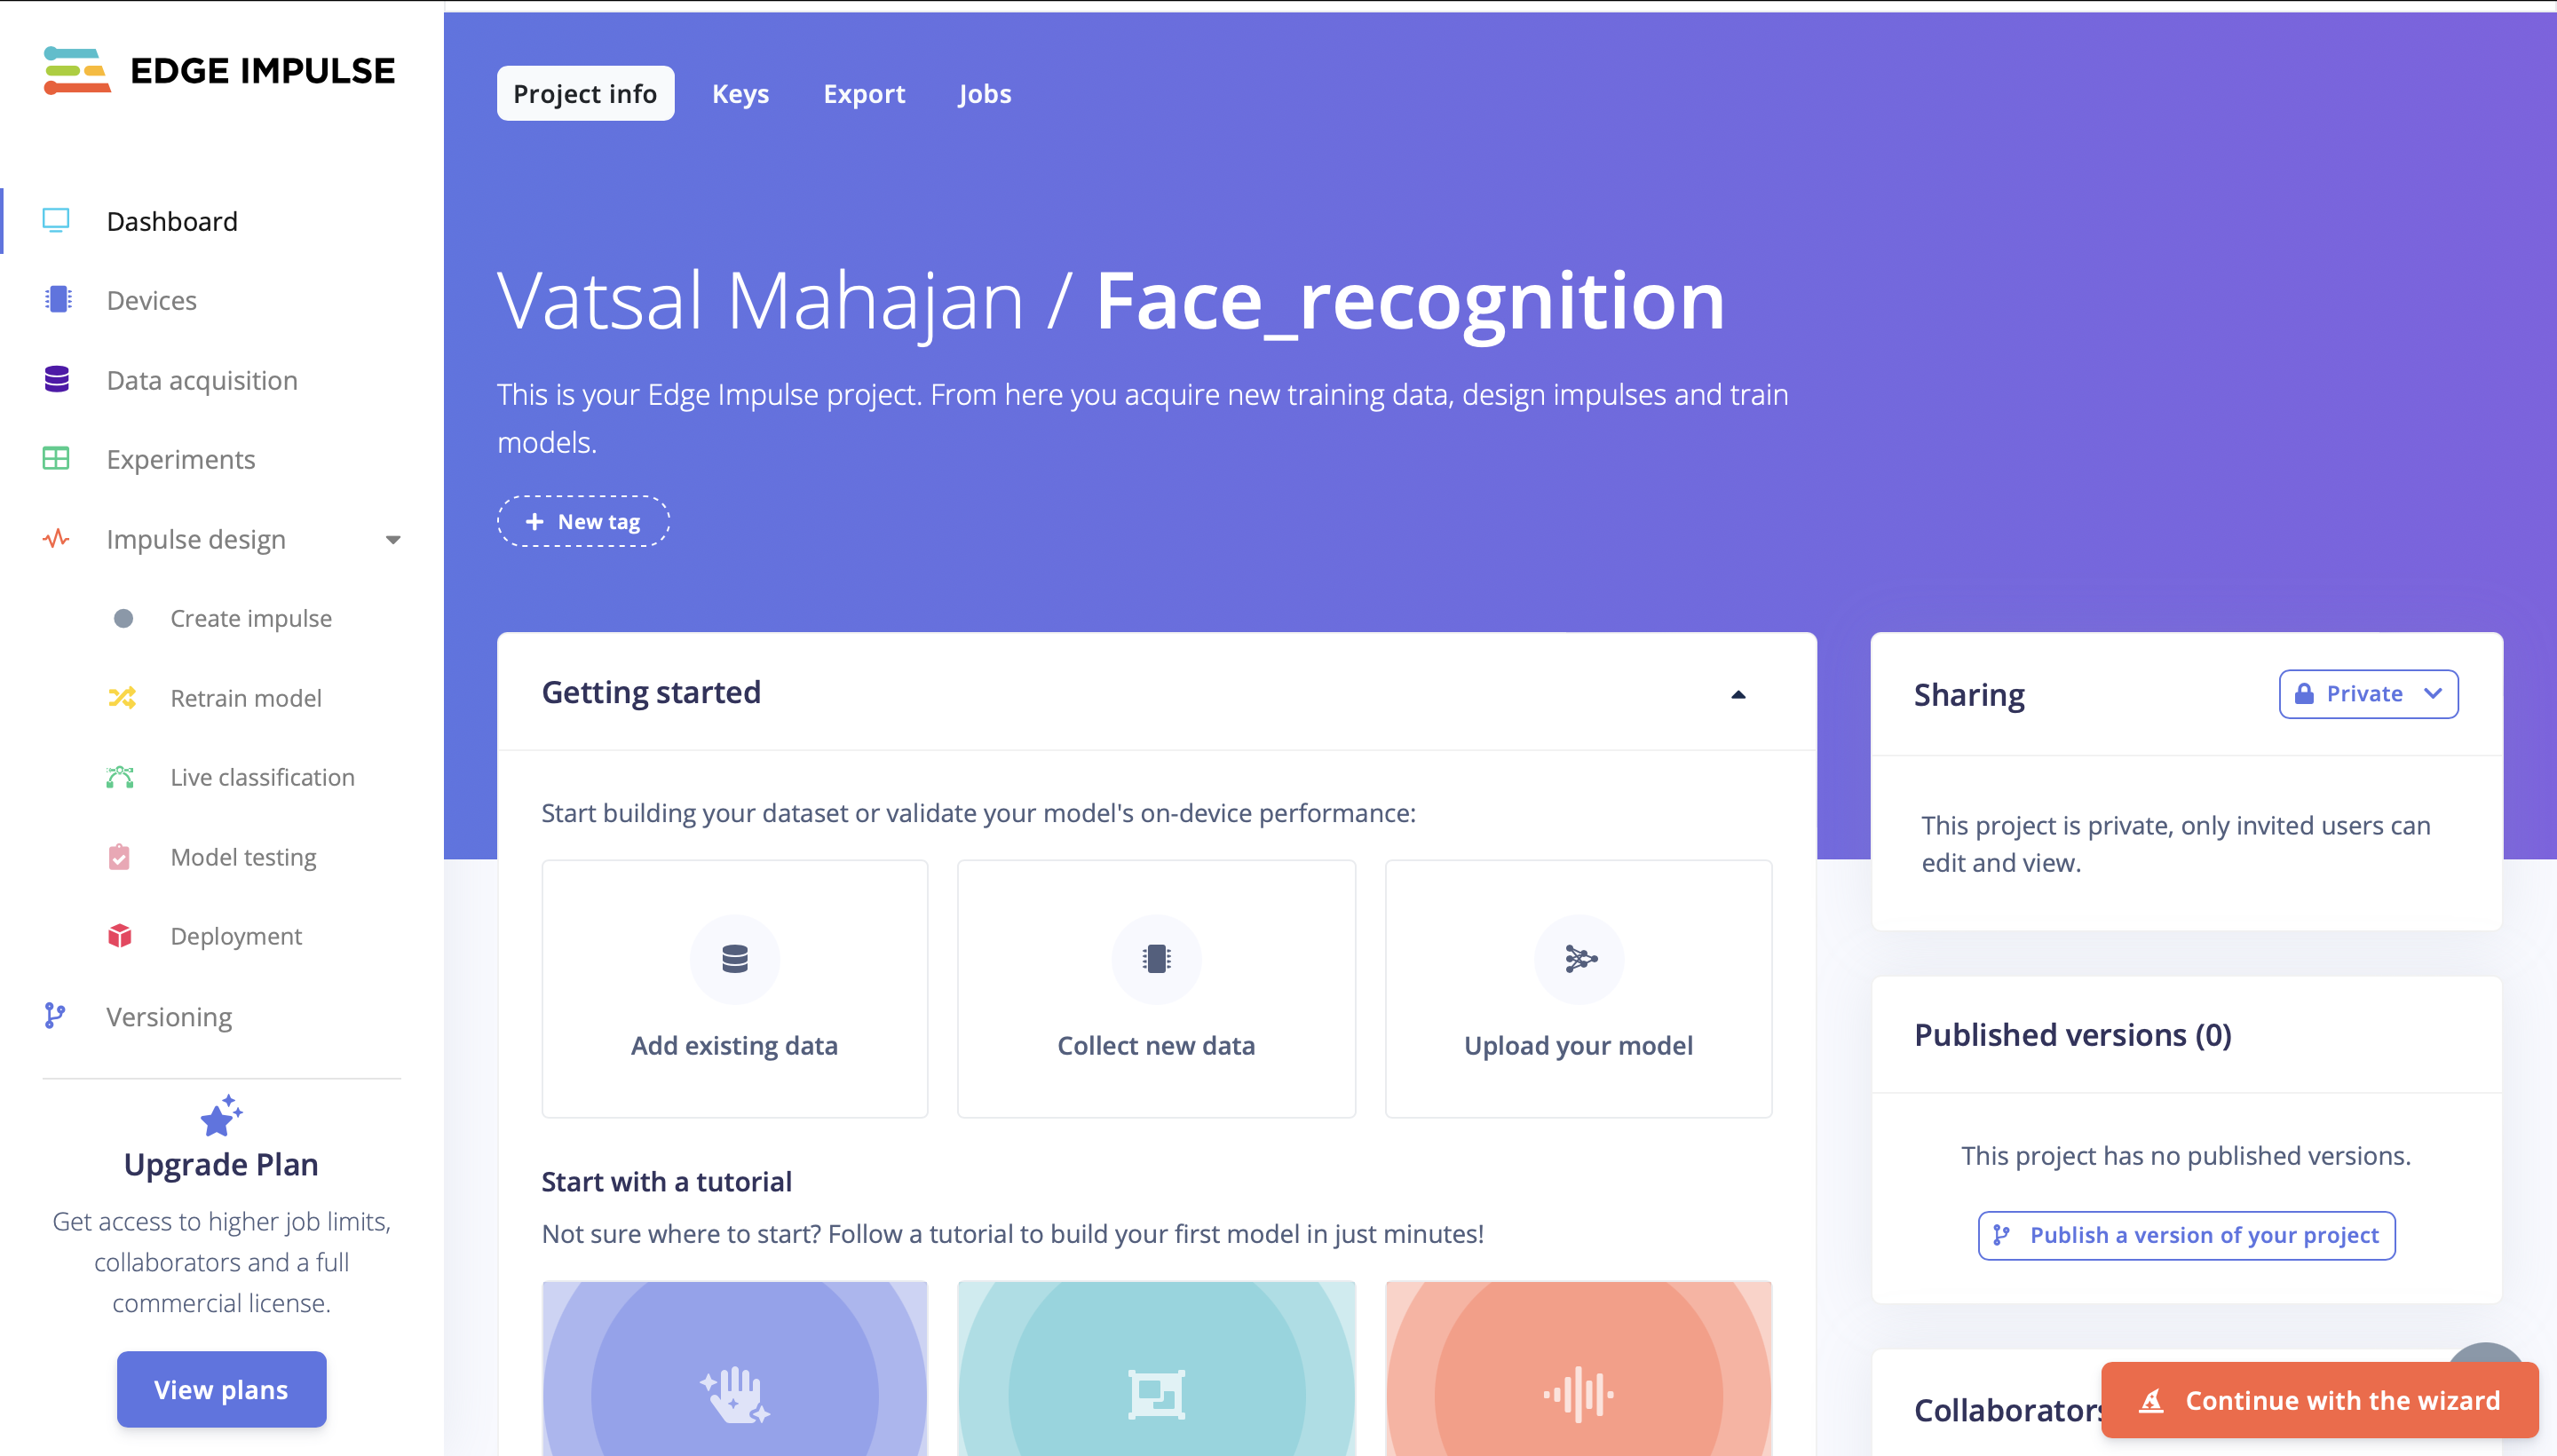
\includegraphics[width=1\textwidth]{images/EdgeImpulse.png}
		\textbf{Figure 1: Edge Impulse}
		
	\end{columns}
\end{block}
\end{frame}
		

	
	\section{Dataset Preparation and Upload}
	\begin{frame}
		
	
		\frametitle{Dataset Preparation and Upload}
		
		\begin{block}{Creating our Own Dataset}
			In the Project we are using our own dataset for the model training and testing.
			\begin{itemize}
				\item We have face images for the three distinct people, organize them in separate folders named Vatsal, Manoj, and Vijay.
				\item To train the model we need the enough images (at least 50-70 per person) under different conditions (lighting, angle) for better performance.
			\end{itemize}
		\end{block}
		
		\begin{block}{Uploading the dataset to Edge Impulse}
			\begin{itemize}
				\item Go to Edge Impulse and log in or create an account.
				\item Create a new project, name it (e.g.,"Face Recognition"), and select Image as the type of data for your project.
				\item Go to the "Data Acquisition" tab: This is where you'll upload your dataset.
				
			\end{itemize}
			
		\end{block}
	\end{frame}
	
	\section{Uploading Images}	
\begin{frame}{Uploading Images}
		\begin{block}{}
			\begin{itemize}
				\item Click on Upload Data. Then drag and drop the images of each person into the platform.
				\item Making sure to label each image accordingly, like Vatsal, Manoj, and Vijay.
		\end{itemize}
			
			\centering
			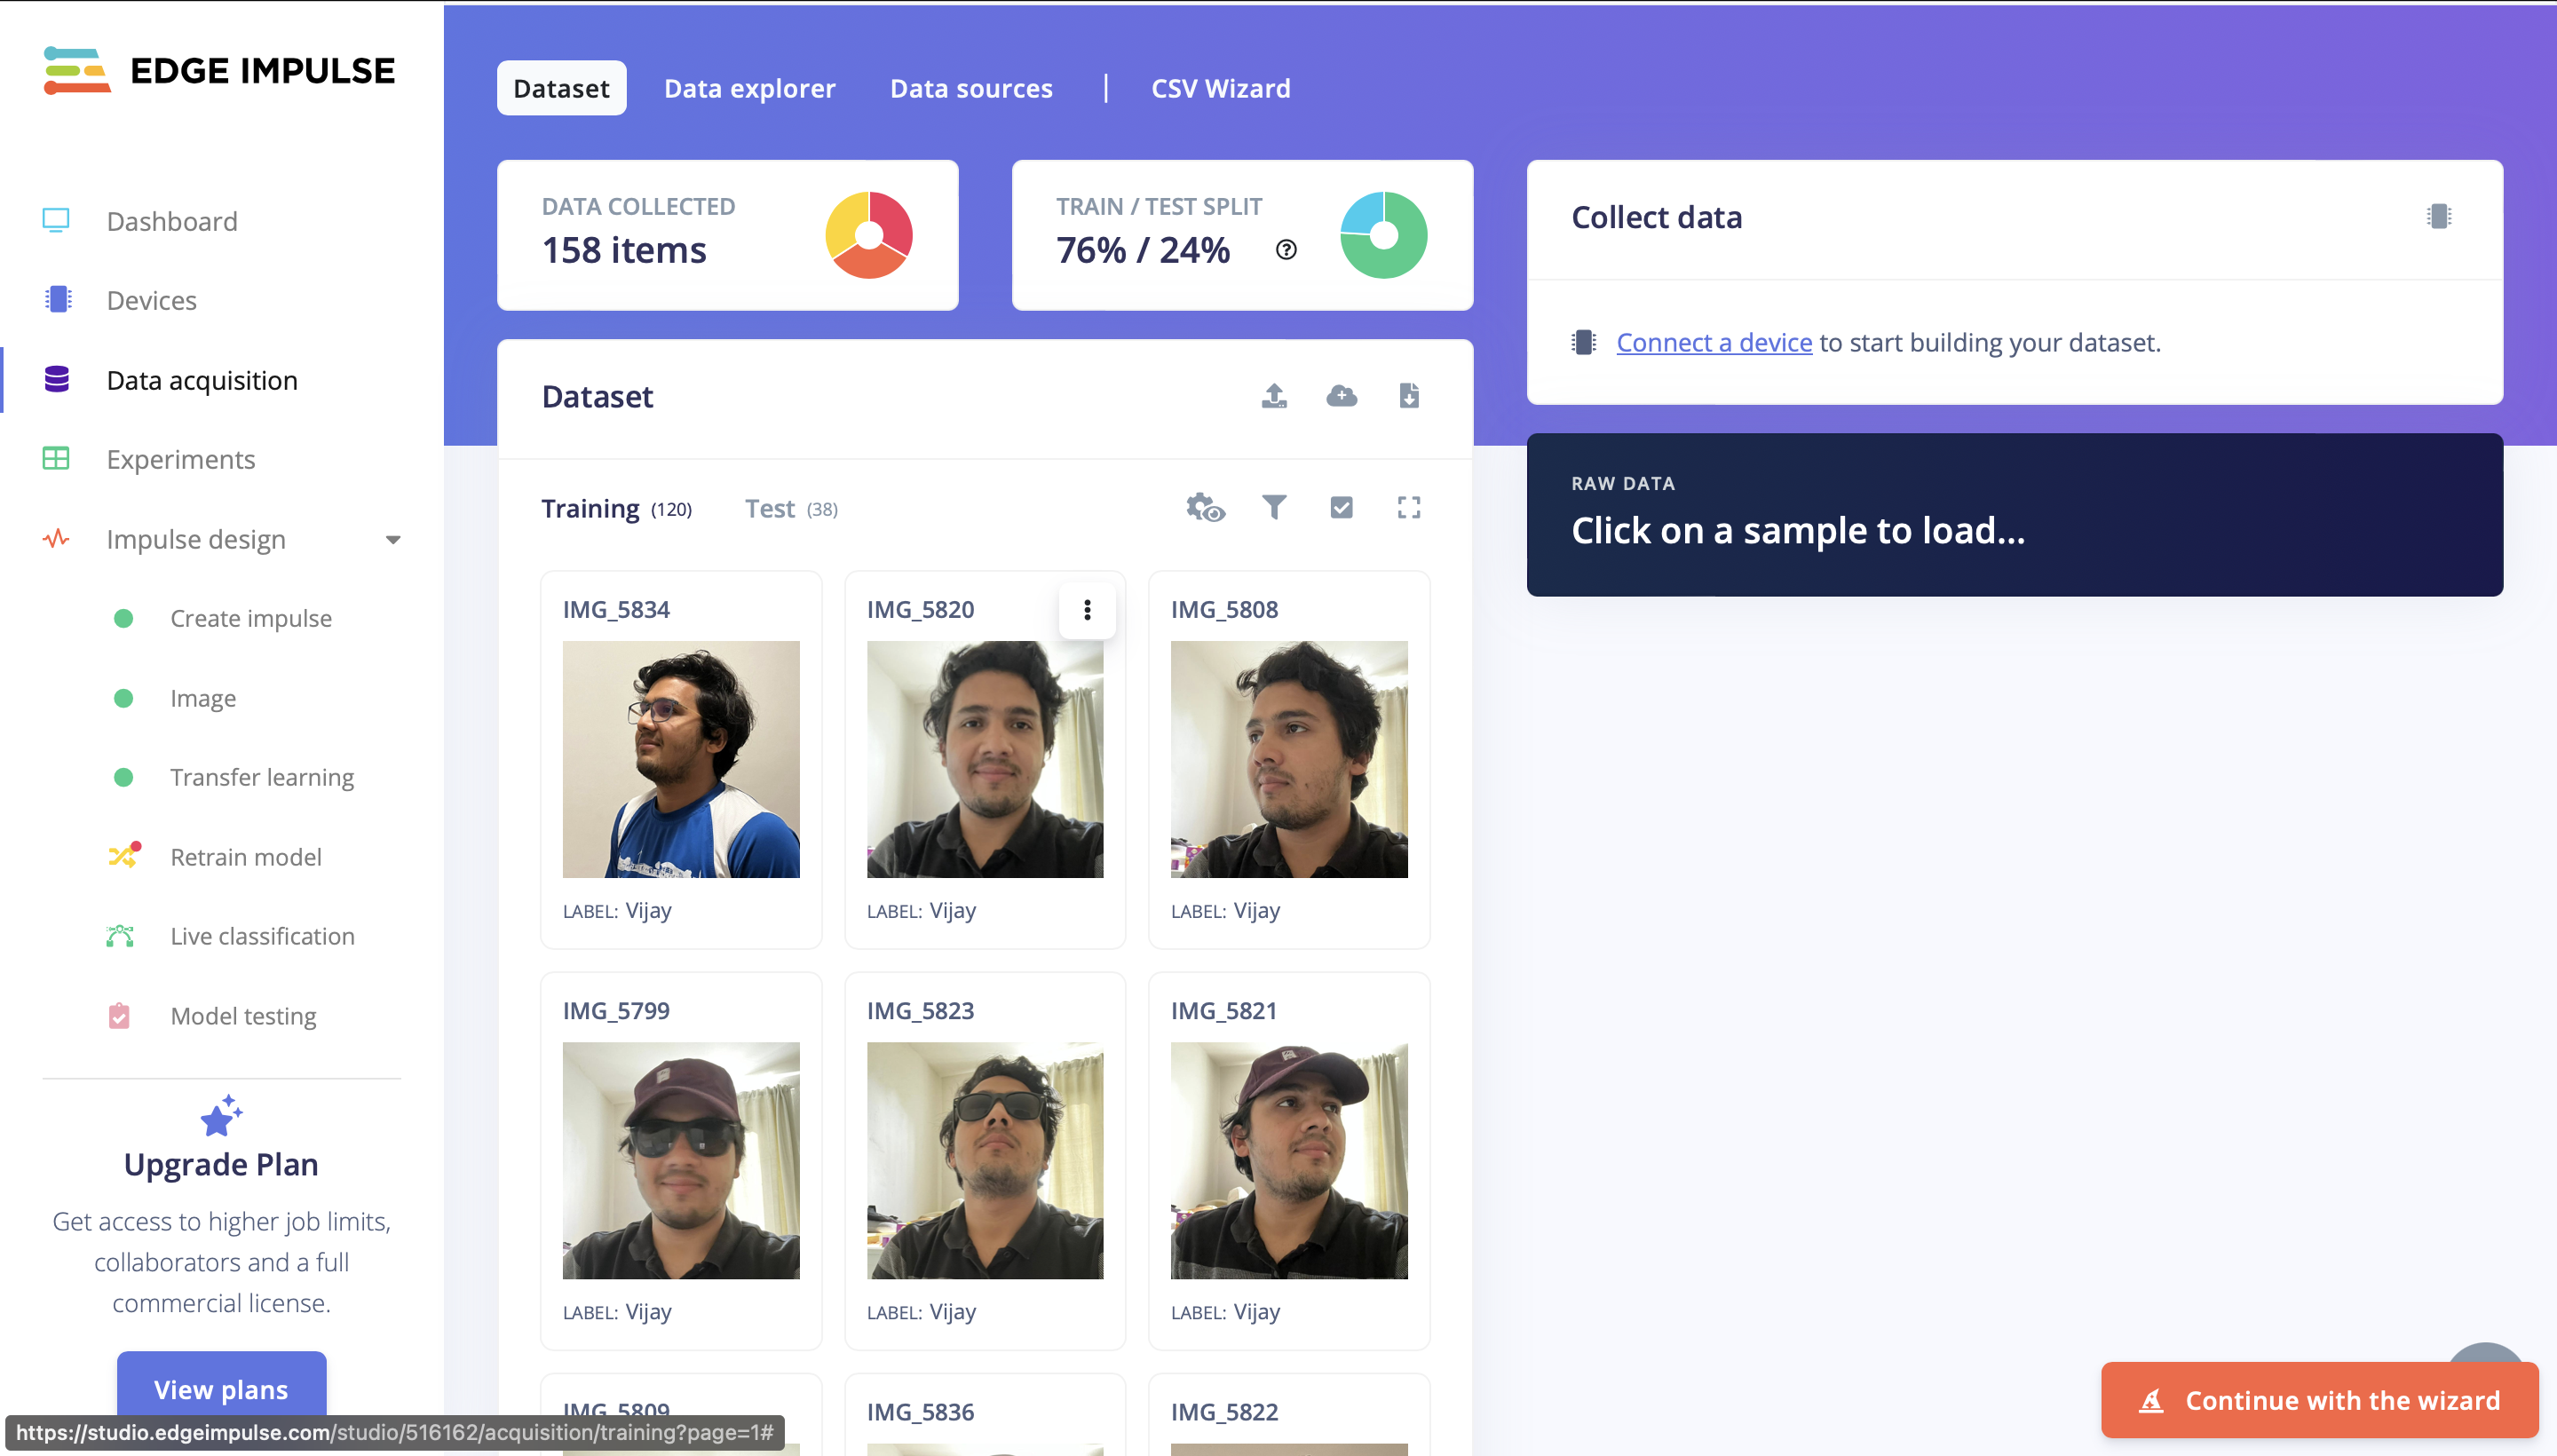
\includegraphics[width=0.9\textwidth]{images/DataSet.png}
			\textbf{Figure 2: Dataset}
			
		\end{block}
\end{frame}

	\section{Impulse Design}
\begin{frame}{Impulse Design}
	Once our dataset is uploaded, we'll design an Impulse (model pipeline) in Edge Impulse.
	
	\begin{block}{Choosing the Model Architecture}
		Model Choice: Convolutional Neural Network (CNN). \\
		For image-related tasks like face recognition, CNNs are typically the best choice. CNNs can detect patterns (like facial features) and differentiate between individuals.
			\begin{itemize}
				\item Click on the Impulse Design tab in Edge Impulse.
				\item Choose the Image block. This will preprocess the images (resize, convert to grayscale if needed, etc.) and prepare them for model input.
				\item Select Image Classification as the task.
				\item Choose a CNN architecture for the project.
				\item We may need to resize our input images to a 320 x 320 pixels resolution to make the model efficient.
			\end{itemize}

\end{block}	
\end{frame}		

\begin{frame}{Impulse Design}
		
		\centering
		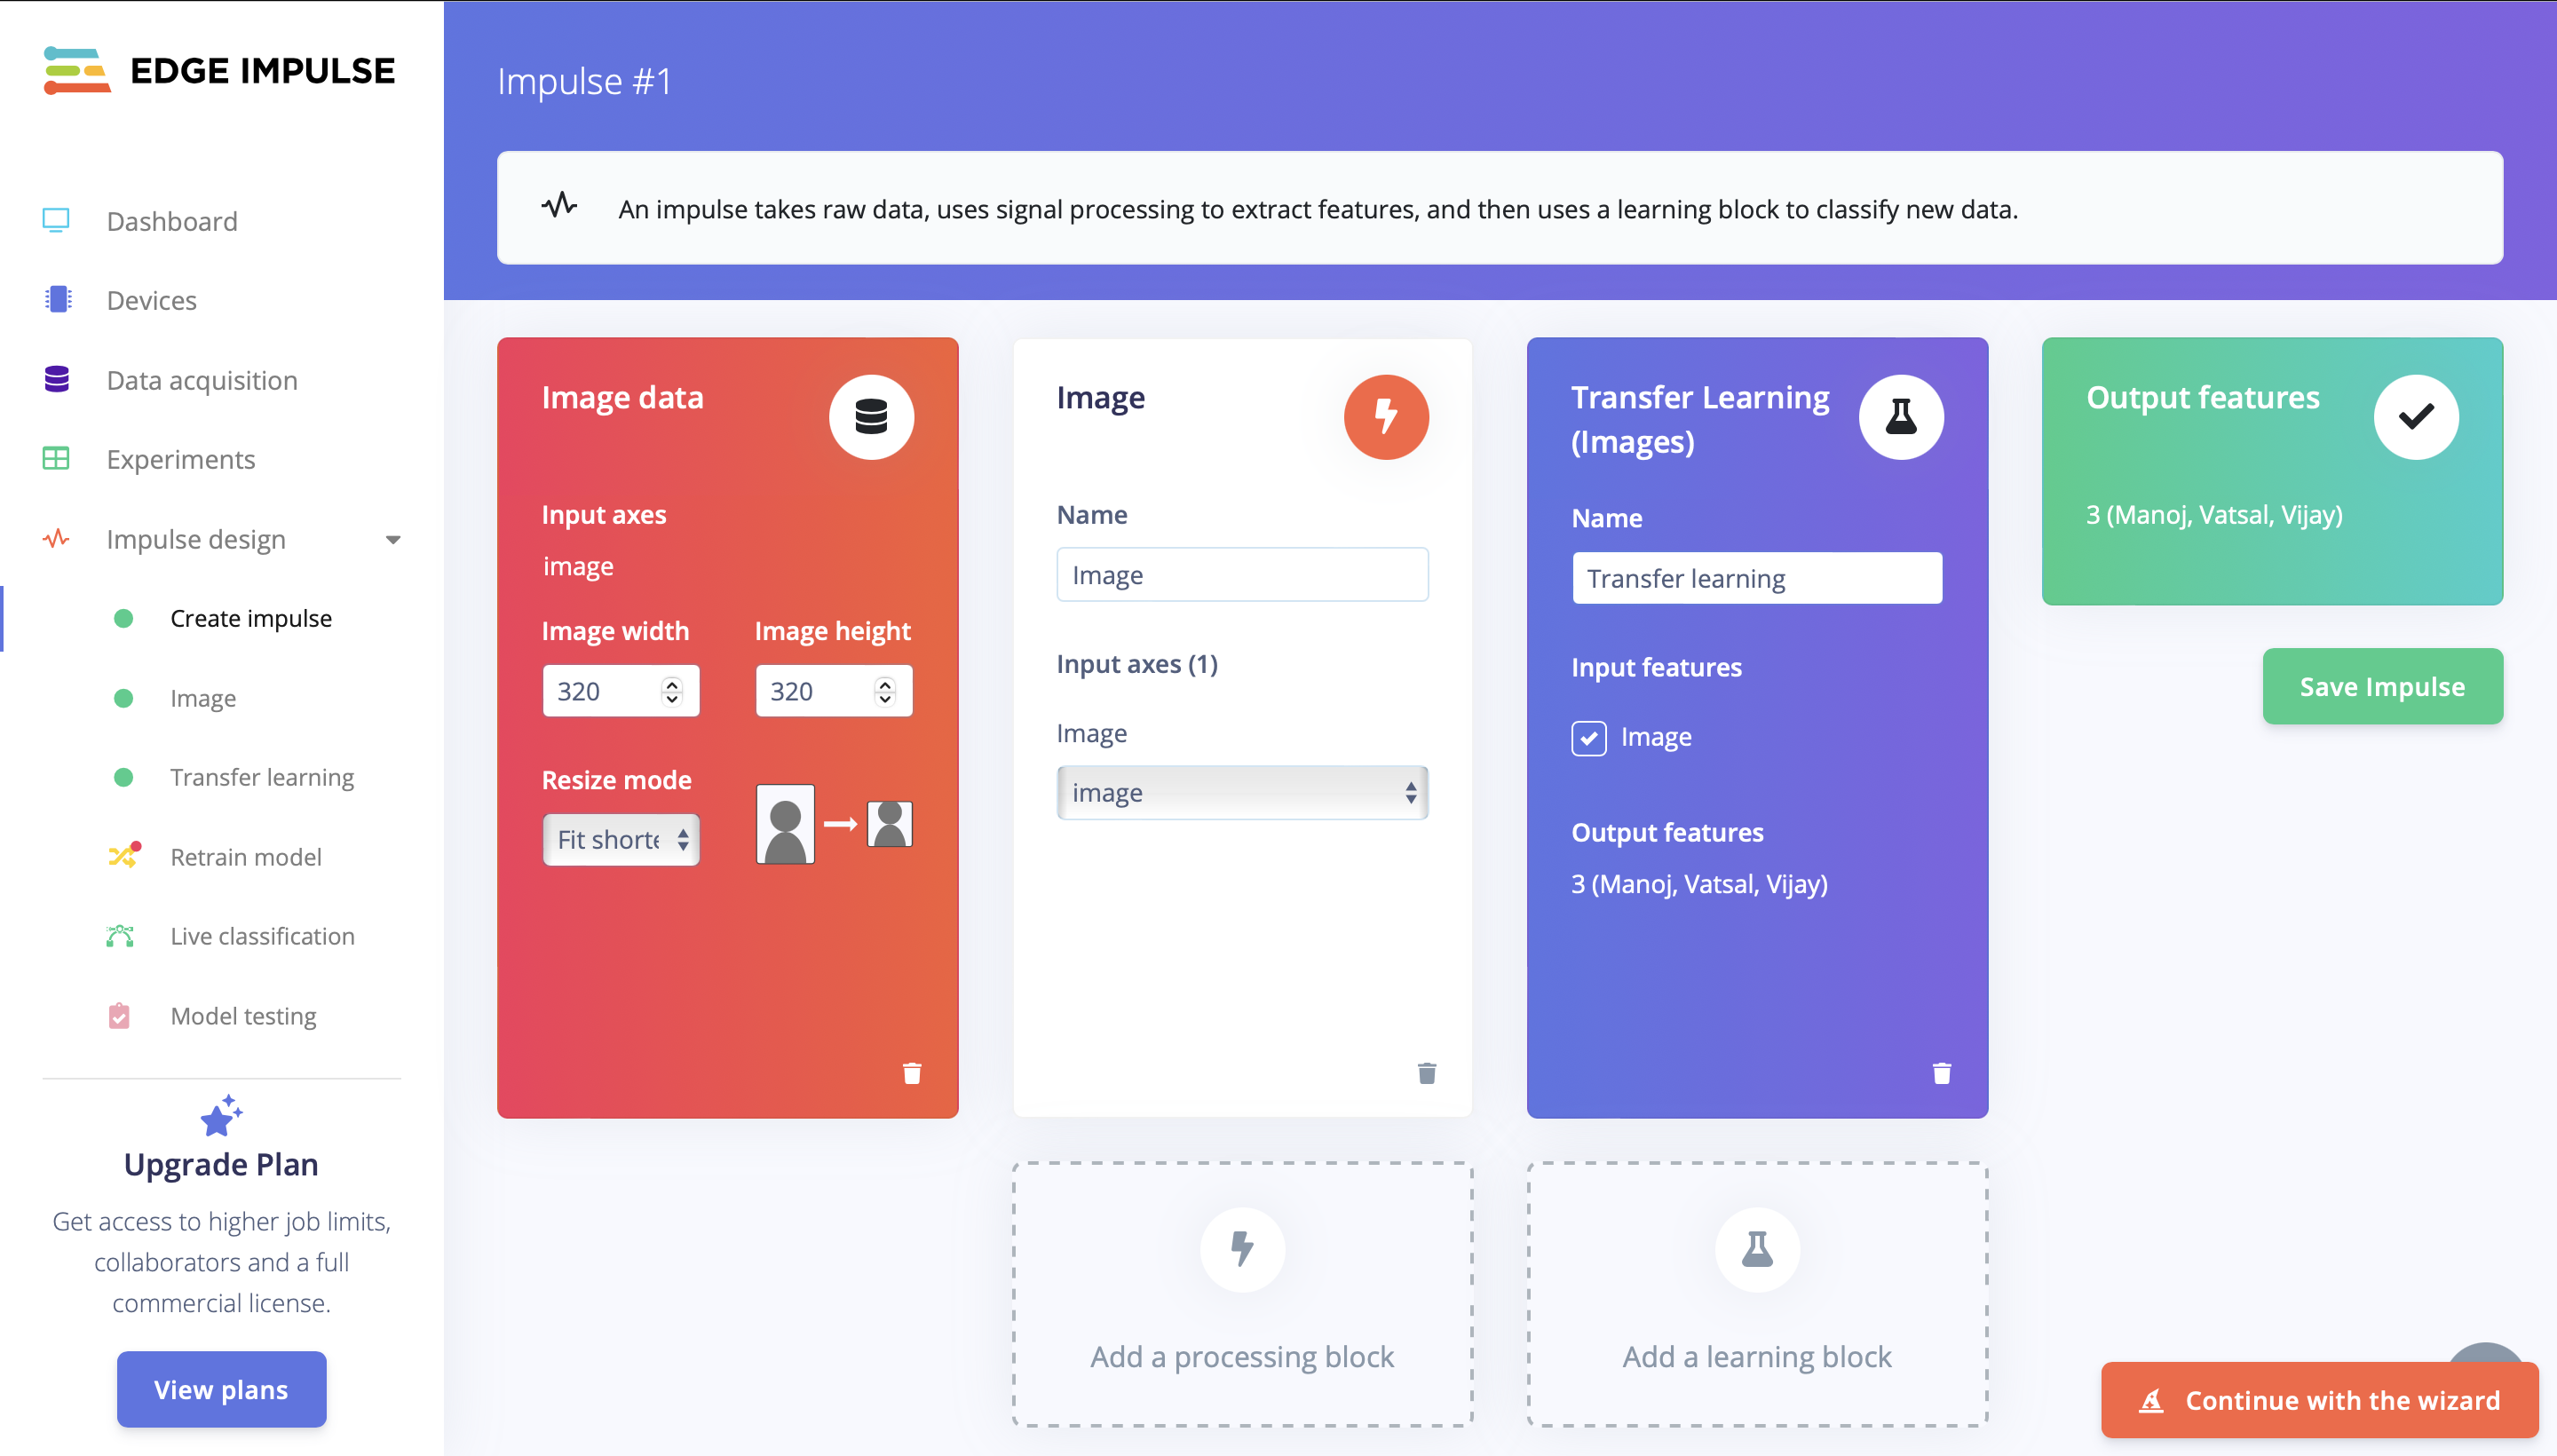
\includegraphics[width=0.9\textwidth]{images/ImpulseDesign.png}
		\textbf{Figure 3: Impulse Design}
	
\end{frame}

	\section{Model Training}
\begin{frame}{Model Training}
	\begin{block}{Configuring Training Parameters}
		\begin{itemize}
			\item \textbf{Training/Validation Split:} Usually 80\% training, 20\% validation. But in our case, it's \textbf{76\%} training, \textbf{24\%} validation.
			\item \textbf{Number of training cycles (Epochs):} 25
			\item \textbf{Learning rate:} 0.0005
		\end{itemize}
	\end{block}
	
	\begin{block}{Model Training}
		\begin{itemize}
			\item \textbf{Accuracy:} 83.3\%
			\item \textbf{Loss:} 0.22
		\end{itemize}
	\end{block}
\end{frame}

\begin{frame}{Model Training}
	
		\centering
	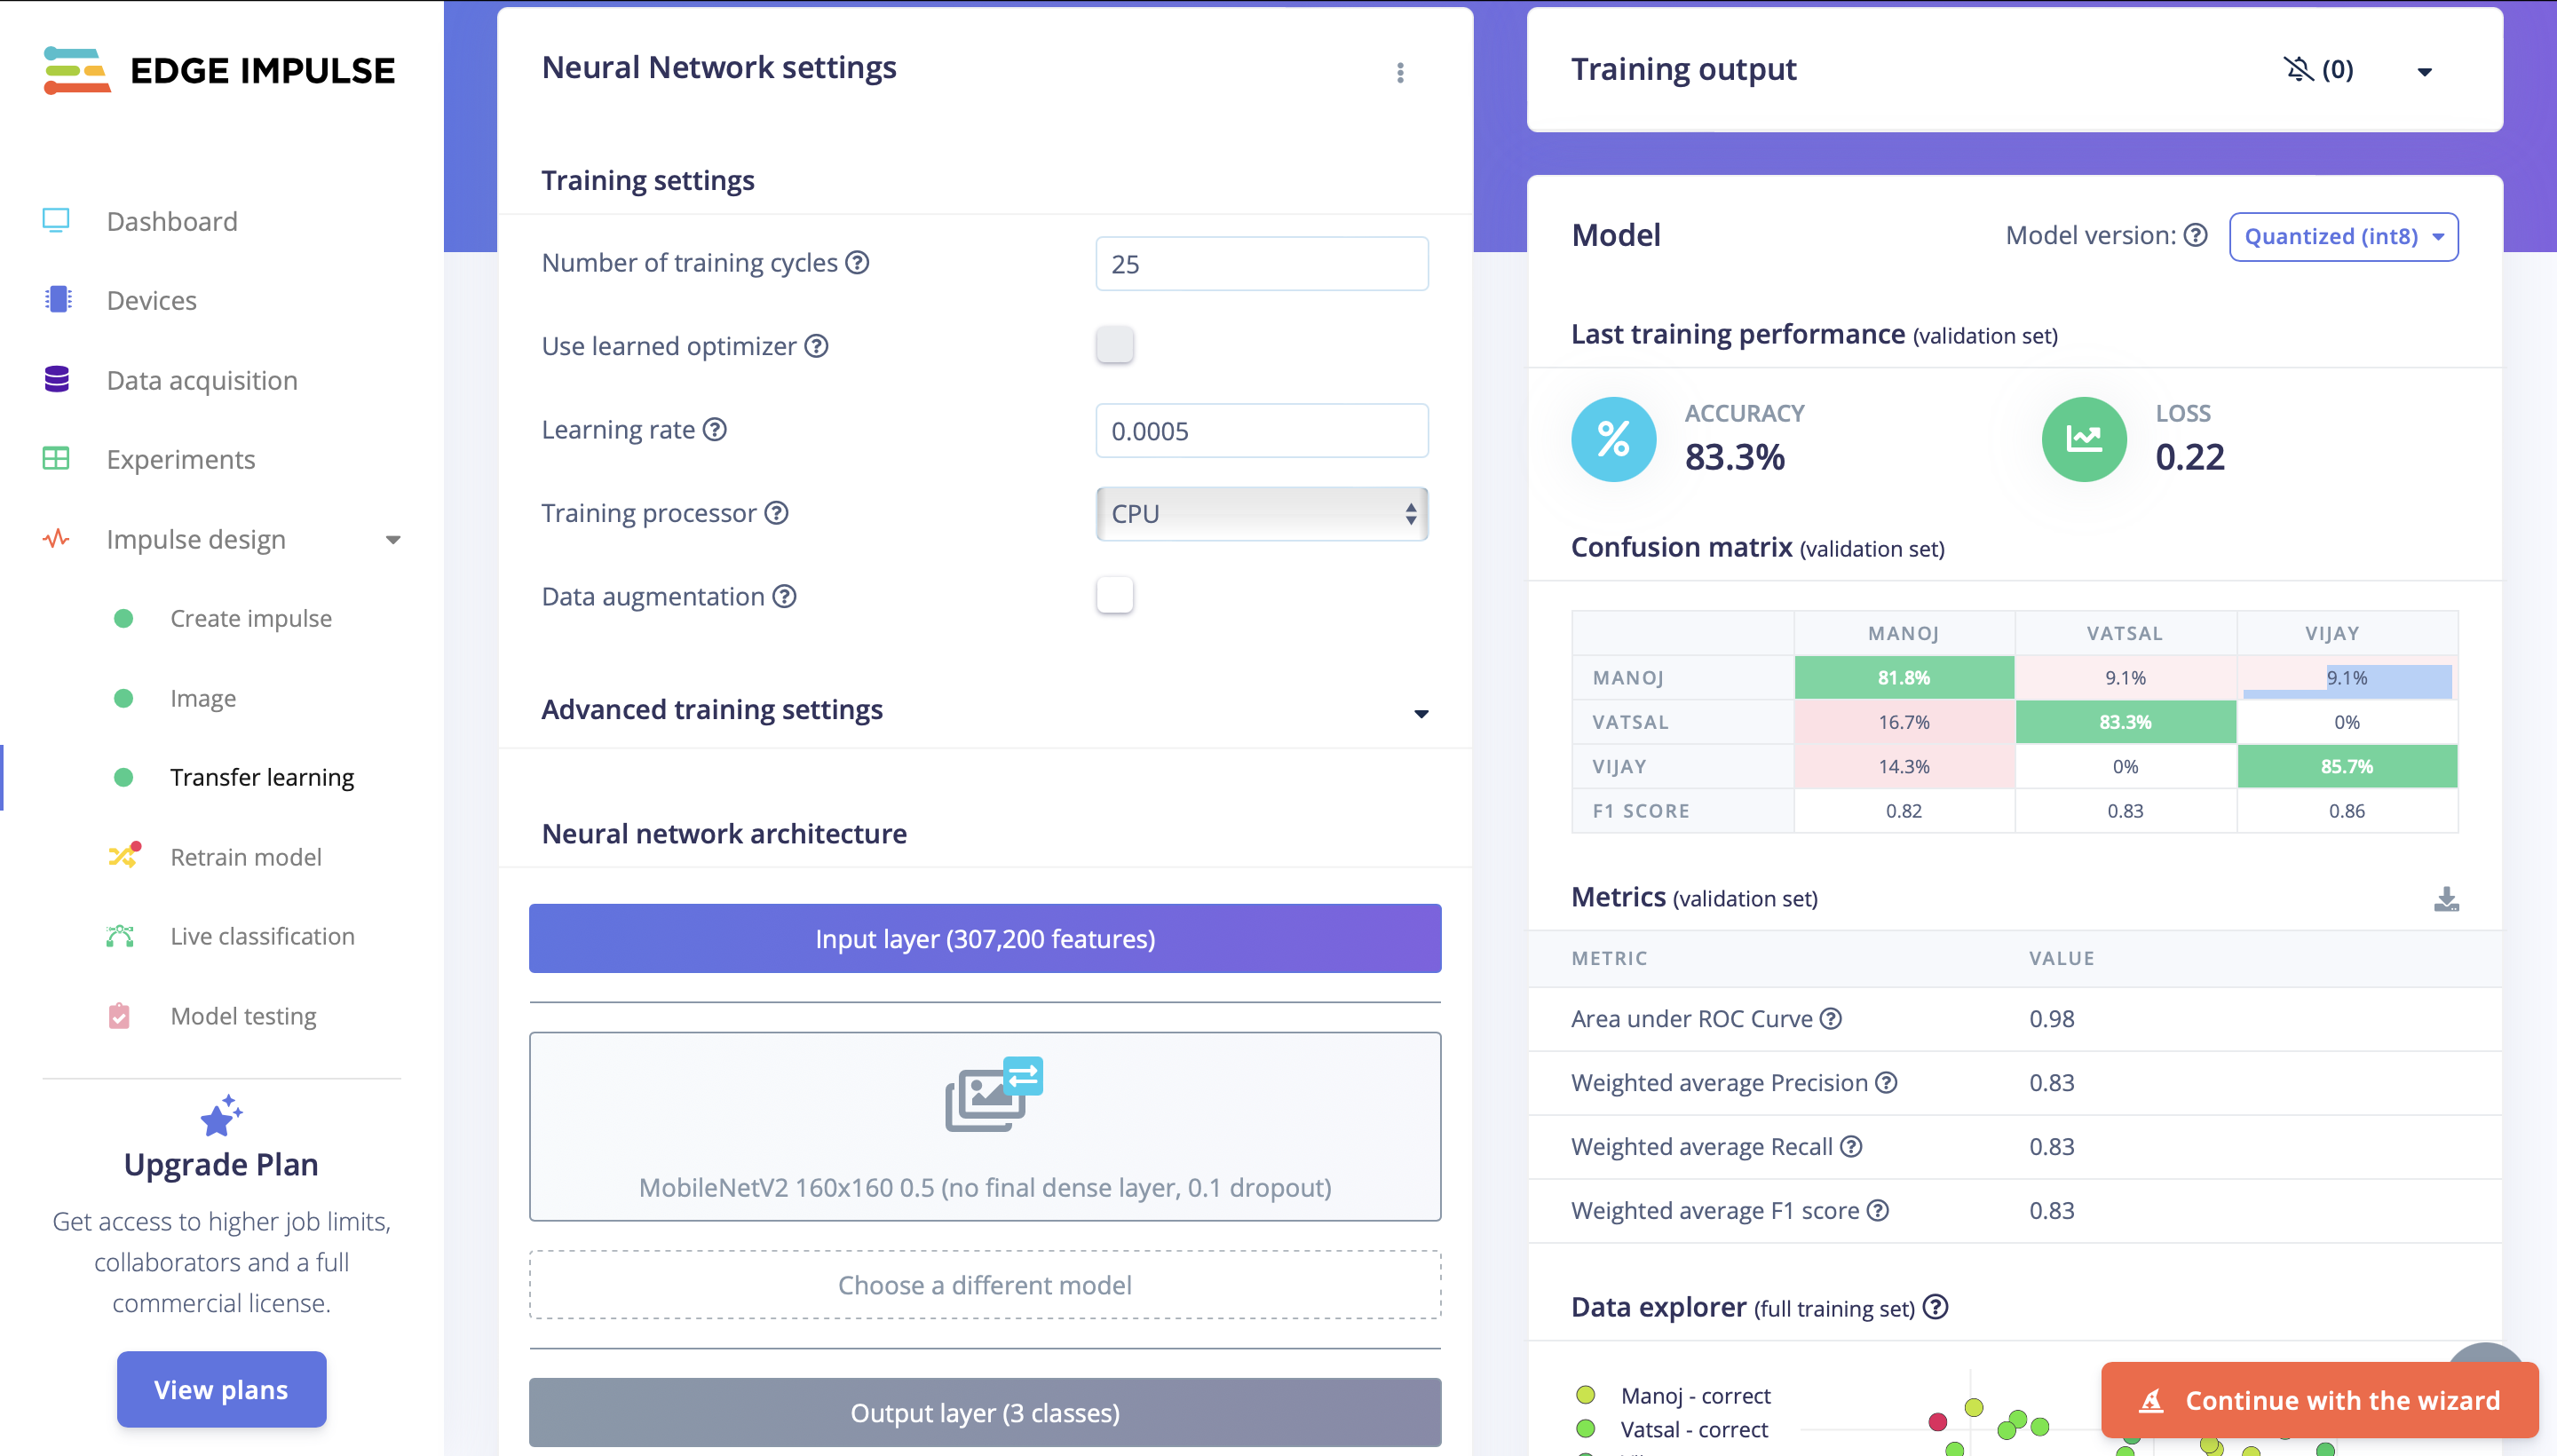
\includegraphics[width=1.0\textwidth]{images/Accuracy.png} % Replace with your image file
	\textbf{Figure 4: Model Training Progress}
	
\end{frame}


	\section{Model Testing}
\begin{frame}{Model Testing}
	\begin{block}{Evaluating the Model}
		\begin{itemize}
			\item  \textbf{To Test the model:} Go to "Live Classification" tab. we uploaded some new images and the model recognizes faces.
			\item  \textbf{Confidence Score:} The system will show confidence scores for each class (Vatsal, Manoj, Vijay).
		\end{itemize}
\end{block}

\centering
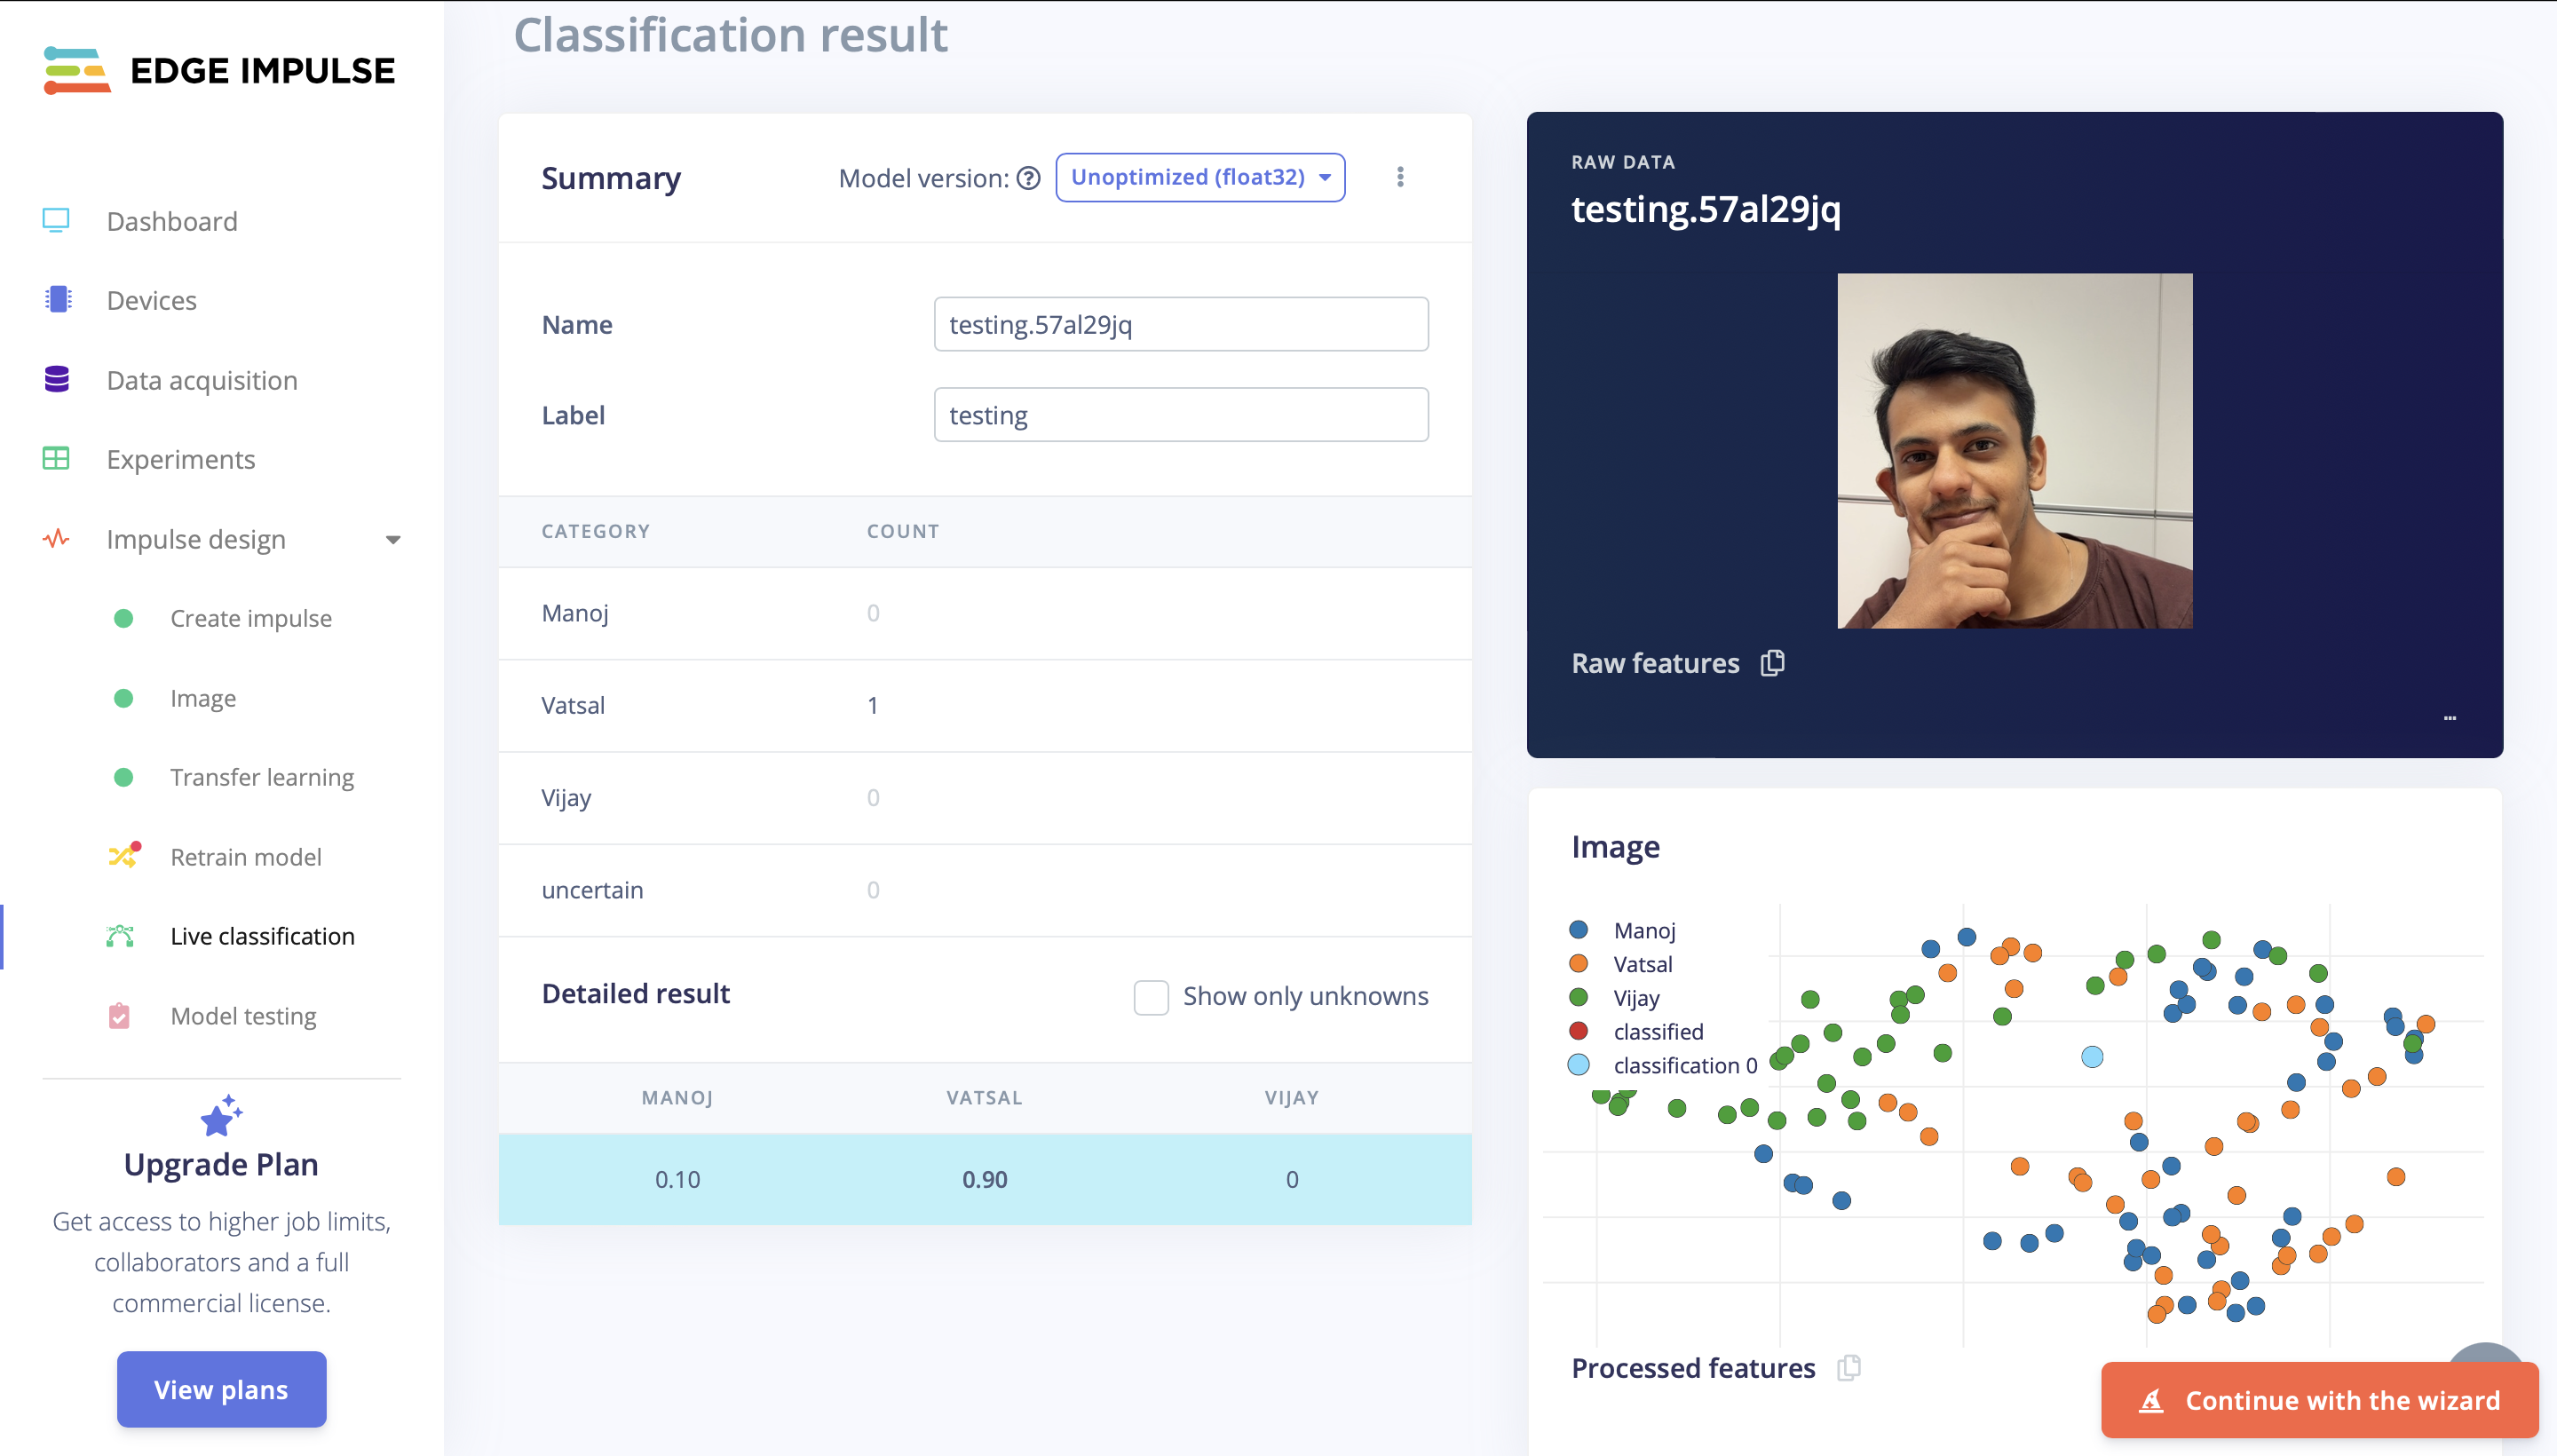
\includegraphics[width=0.8\textwidth]{images/Test.png} 

\end{frame}


	\section{Model Deployment}
\begin{frame}{Model Deployment}
	\begin{block}{Evaluating the Model}
		\begin{itemize}
		 \item Go to the Deployment tab.
		 \item Select \textbf{TensorFlow Lite (.tflite)} as the export format.
		 \item \textbf{Quantization:} Choose \textbf{int8 Quantization} if you plan to run the model on embedded systems like Portenta H7. Quantization reduces the model size and speeds up inference.
			
		\end{itemize}
\end{block}
\end{frame}

\STANDARD{}
{
  \begin{columns}
    \begin{column}{0.35\textwidth}
      \begin{block}{~~~~~~Thank you}
        \centering
        for your attention
      \end{block}
    \end{column}
  \end{columns}
}

\MYNOTE{Ja, \textbf{Vielen} Dank, für Ihre Aufmerksamkeit}


	
\end{document}
